\section{MOSFET and BJT}
\subsection{MOSFET}
\subsubsection*{Scheme}
A MOSFET (Metal-Oxide-Semiconductor Field-Effect Transistor) is a three-terminal semiconductor device that can be used as
a switch. It has three terminals: Gate (G), Drain (D) and Source (S). The current flowing from Drain to Source (\(I_{DS}\))
is controlled by the voltage applied to the Gate (\(V_{GS}\)).

\begin{center}
	\begin{minipage}{0.45\textwidth}
		\centering \begin{circuitikz}[american]
			\ctikzset{tripoles/mos style=arrows}
			
			% nmos transistor and terminal labels
			\draw (0,0) node[nmos, scale=1.5] (nmos) {};
			\node[left=0cm] at (nmos.G) {Gate};
			\node[above=0.1cm] at (nmos.D) {Drain};
			\node[below=0cm] at (nmos.S) {Source};
	
			% V_GS (Gate-Source Voltage)
			\draw[-{Latex}]
				([xshift=-0.6cm, yshift=-0.25cm] nmos.S) to[out=180, in=270] 
				node[midway, fill=white, inner sep=4pt] {$V_{GS}$} 
				([xshift=-0.4cm, yshift=-0.25cm] nmos.G);
			
			% V_DS (Drain-Source Voltage)
			\draw[-{Latex}]
				([xshift=0.3cm, yshift=-0.1cm] nmos.S) to[out=60, in=-60] 
				node[midway, fill=white, inner sep=4pt] {$V_{DS}$} 
				([xshift=0.3cm, yshift=0.1cm] nmos.D);
		
			% I_DS Drain-Source current
			\node at ($(nmos.D)+(-0.5, -0.2)$) {\(I_{DS} \downarrow\)};
		\end{circuitikz} \\[5pt]
		NMOS transistor
	\end{minipage}
	\begin{minipage}{0.45\textwidth}
		\centering \begin{circuitikz}[american]
			\ctikzset{tripoles/mos style=arrows}
			\ctikzset{tripoles/pmos style/emptycircle}
			
			% PMOS transistor and terminal labels
			\draw (0,0) node[pmos, scale=1.5] (pmos) {};
			\node[left=0cm] at (pmos.G) {Gate};
			\node[below=0.1cm] at (pmos.D) {Drain};
			\node[above=0cm] at (pmos.S) {Source};
	
			% V_GS (Gate-Source Voltage)
			\draw[-{Latex}]
				([xshift=-0.4cm, yshift=0.25cm] pmos.G) to[out=90, in=180] 
				node[midway, fill=white, inner sep=4pt] {$V_{GS}$} 
				([xshift=-0.6cm, yshift=0.25cm] pmos.S);

			% V_DS (Drain-Source Voltage)
			\draw[-{Latex}]
				([xshift=0.3cm, yshift=0.1cm] pmos.D) to[out=60, in=-60] 
				node[midway, fill=white, inner sep=4pt] {$V_{DS}$} 
				([xshift=0.3cm, yshift=-0.1cm] pmos.S);
		
			% I_DS Drain-Source current
			\node at ($(pmos.D)+(-0.5, 0.2)$) {\(I_{DS} \uparrow\)};
		\end{circuitikz}\\[5pt]
		PMOS transistor
	\end{minipage}
\end{center}

\subsubsection*{Operation regions of a NMOS transistor}
\begin{itemize}
	\item \textbf{cutoff region}: \(V_{GS} < V_{TN}\), the MOSFET is off and \(I_{DS} = 0\)
	\item \textbf{linear region}: \(V_{GS} > V_{TN}\) and \(V_{DS} < V_{GS} - V_{TN}\), the MOSFET is on and behaves like a
	gate-voltage controlled resistor, \(I_{DS}\) increases linearly with \(V_{DS}\):
	\[I_{DS} = k_n V_{DS} \left(V_{GS} - V_{TN} - V_{DS}/2\right) \qquad\qquad k_n = \frac{\mu_n \varepsilon}{T_{OX}} \frac{W}{L}\]
	\item \textbf{saturation region}: \(V_{GS} > V_{TN}\) and \(V_{DS} > V_{GS} - V_{TN}\), the MOSFET is on and behaves like a
	gate-voltage controlled current source, \(I_{DS}\) is independent from \(V_{DS}\) and increases quadratically with \(V_{GS}\):
	\[I_{DS} = \frac{k_n}{2} \left(V_{GS} - V_{TN}\right)^2 \qquad\qquad k_n = \frac{\mu_n \varepsilon}{T_{OX}} \frac{W}{L}\]
\end{itemize}
There are some non-idealities for short channel length transistors that affect the behavior of the MOSFET:
\begin{itemize}
	\item \textbf{pinch-off saturation region - channel length modulation}: in saturation region, the effective channel length decreases as \(V_{DS}\) increases
	and the current \(I_{DS}\) increases slightly with \(V_{DS}\) instead of being constant by a factor \(\lambda\) (channel length
	modulation parameter):
	\[I_{DS} = \frac{k_n}{2} \left(V_{GS} - V_{TN}\right)^2 \left(1 + \lambda V_{DS}\right)\]
\end{itemize}

\begin{center}
	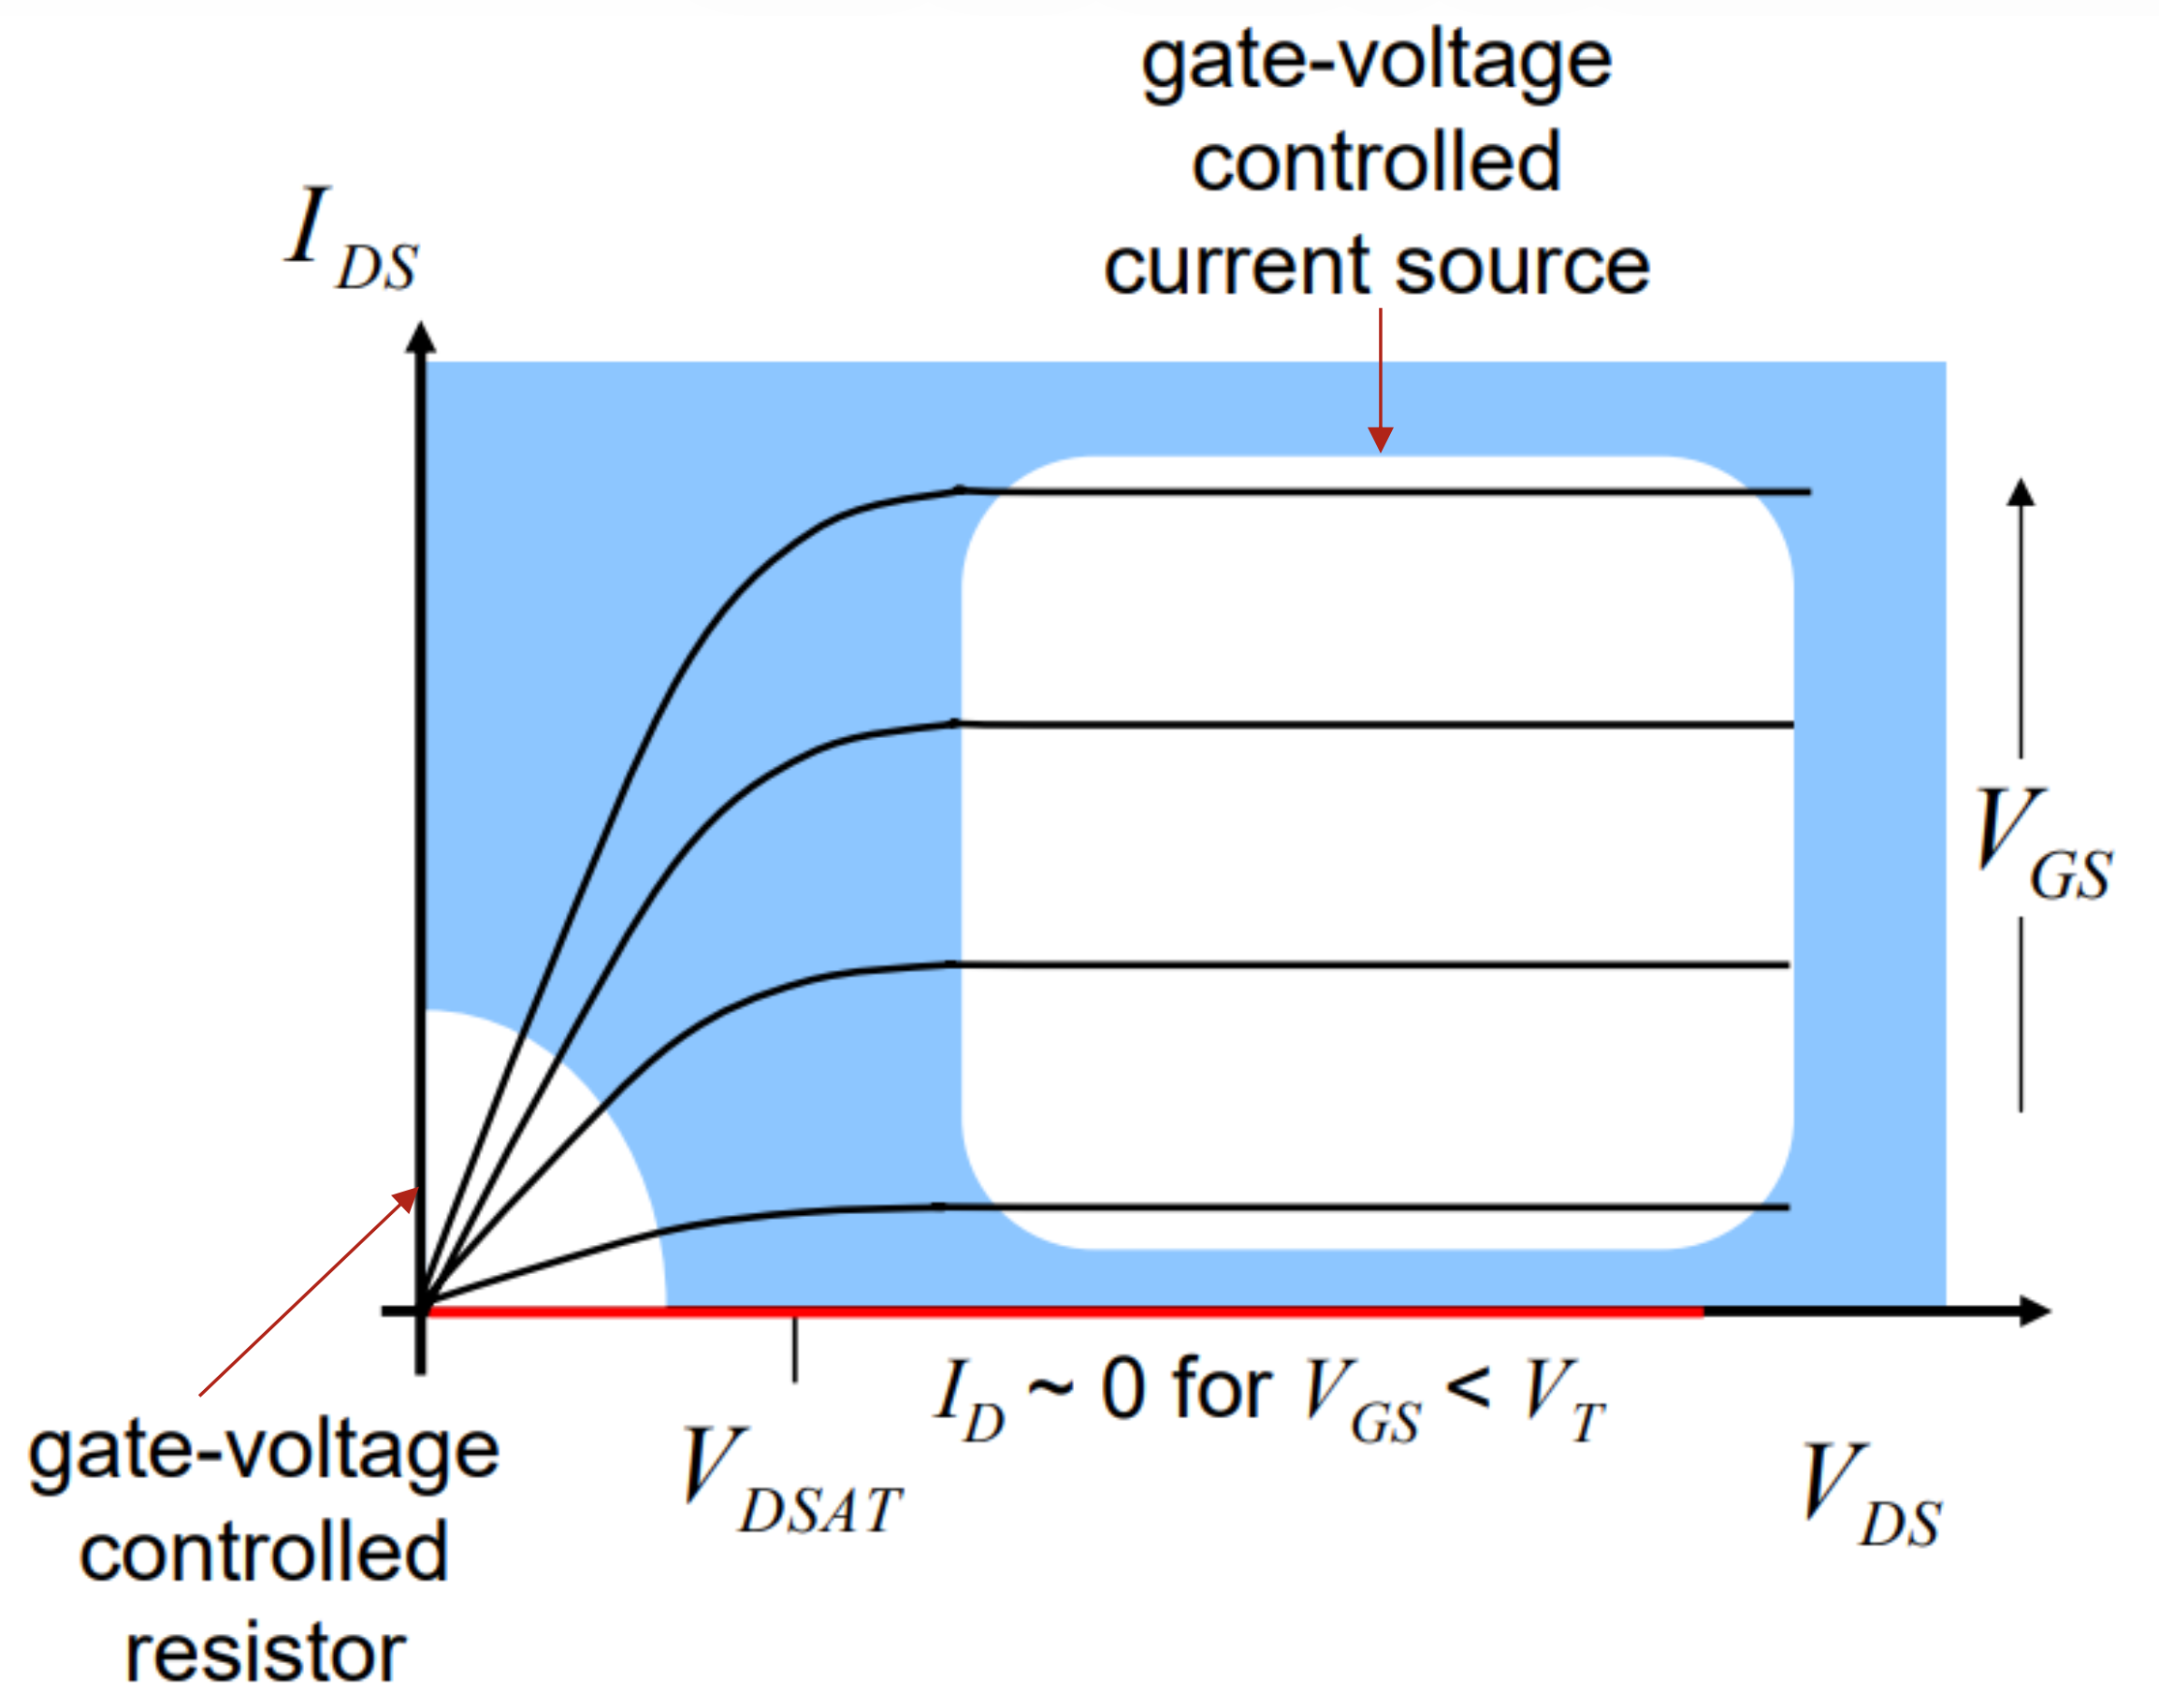
\includegraphics[width=0.5\textwidth]{immagini/nmos_characteristics.png}
\end{center}

\subsection{BJT}
\subsubsection*{Scheme}
A BJT (Bipolar Junction Transistor) is a three-terminal semiconductor device that can be used as a switch or as a current amplifier.
It is made of three layers of semiconductor material: the emitter (E), the base (B) and the collector (C). The current flowing from
collector to emitter (\(I_{CE}\)) is controlled by the current flowing into the base (\(I_B\)).

\begin{center}
	\begin{minipage}{0.45\textwidth}
		\centering 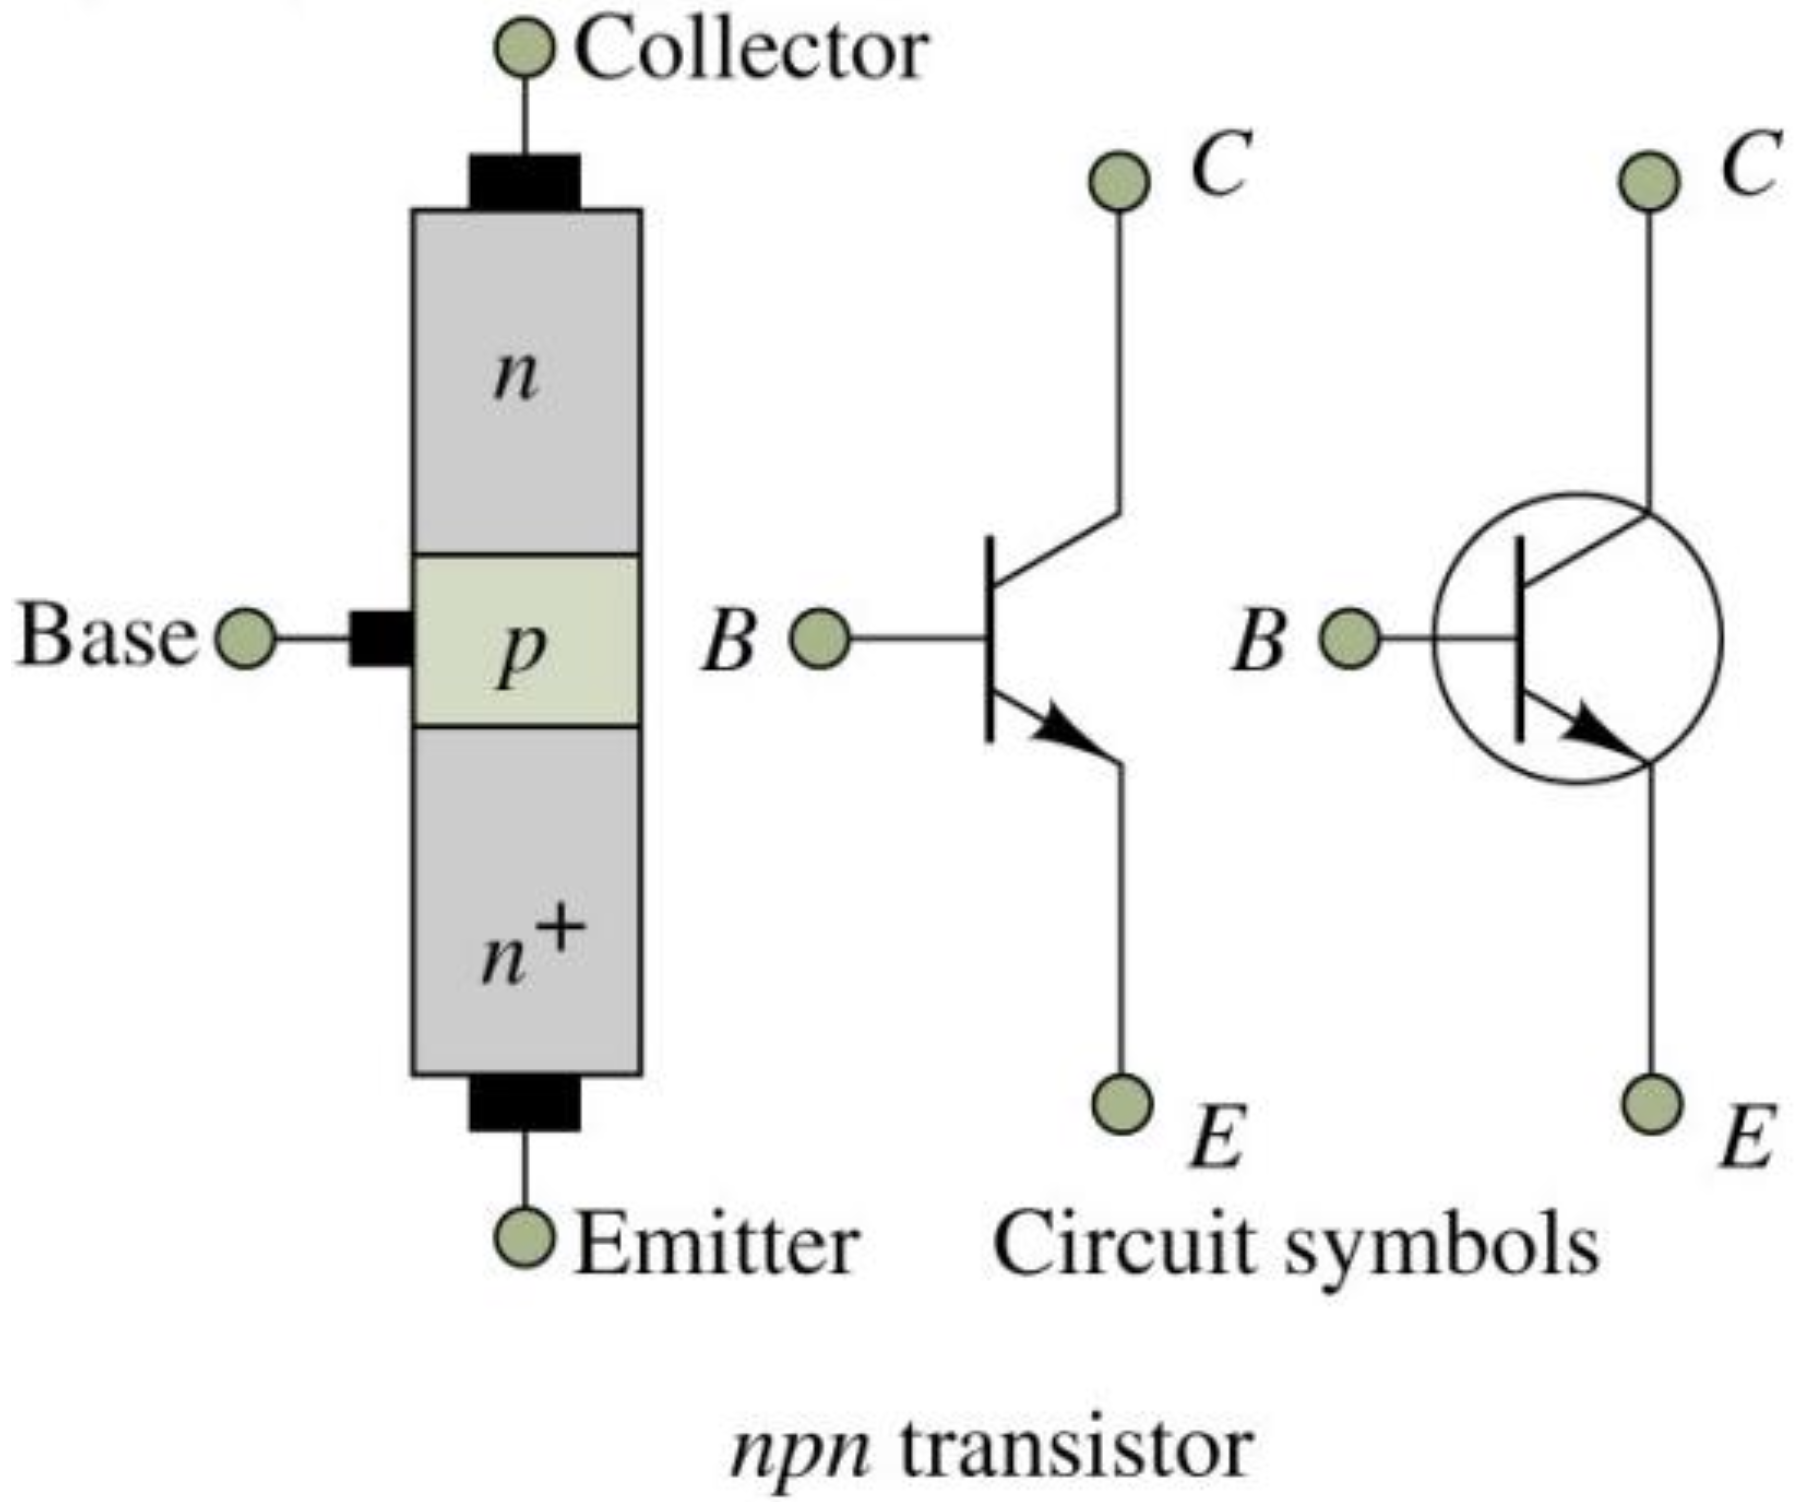
\includegraphics[width=0.8\textwidth]{immagini/npn_bjt.png}
	\end{minipage}
	\begin{minipage}{0.45\textwidth}
		\centering 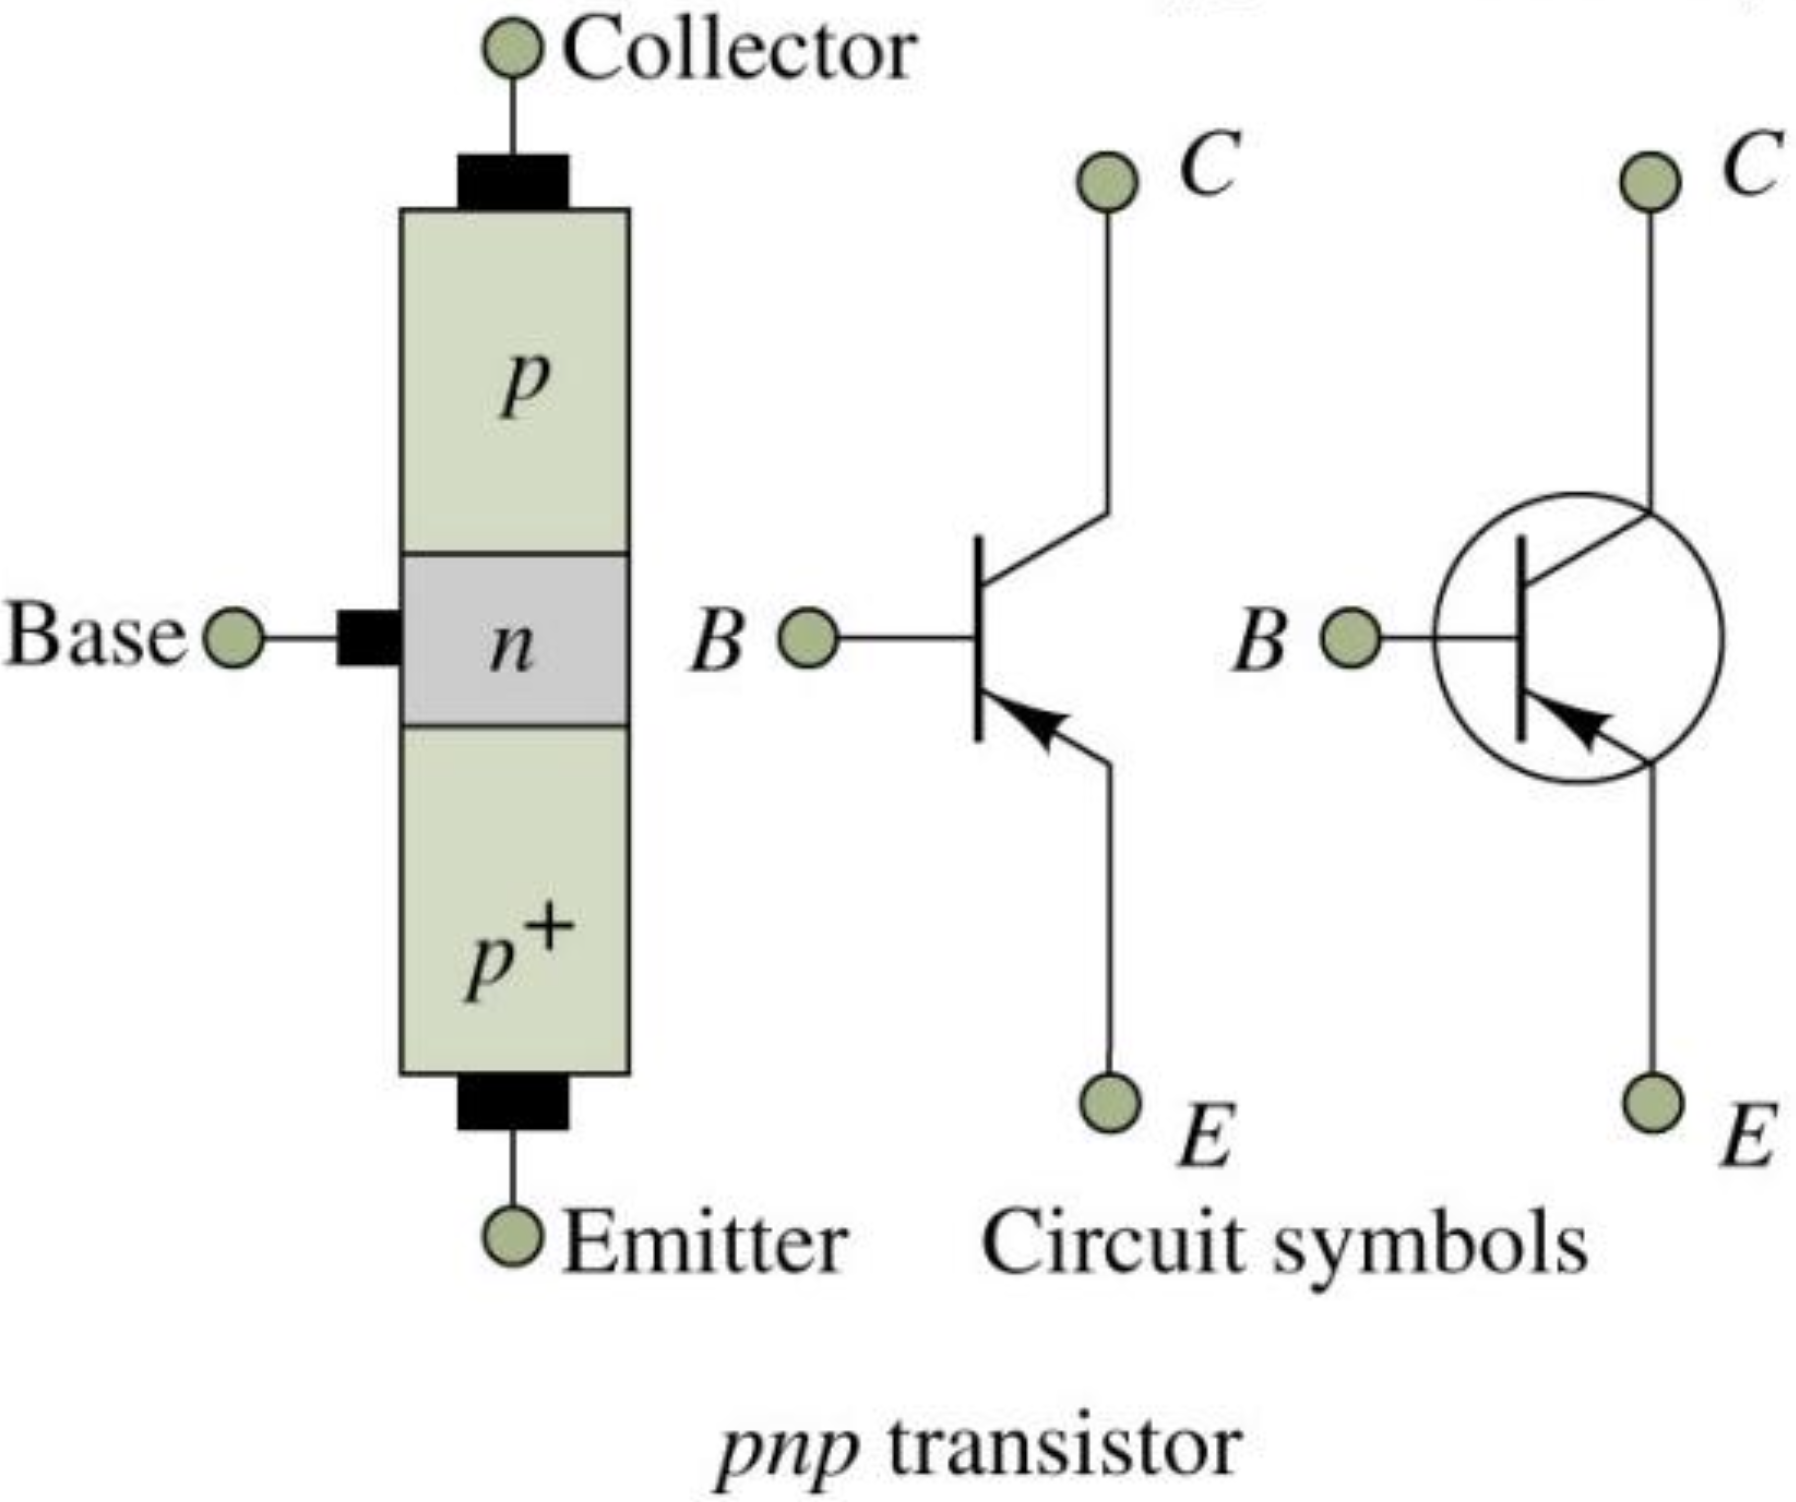
\includegraphics[width=0.8\textwidth]{immagini/pnp_bjt.png}
	\end{minipage}
\end{center}

\subsubsection*{Open Collector Curve}
When the base-emitter junction is forward biased and the collector is not connected to any voltage source (open collector), the BJT
behaves like a diode between the base and the emitter, with a voltage drop of about 0.7 V for silicon BJTs. There is an exponential
dependence between the base current \(I_B\) and the collector-emitter voltage \(V_{CE}\) (the same characteristic of a diode).
\[I_B = I_S \left(\exp \left( \frac{V_{BE}}{\eta V_T}\right) - 1\right)\]

\subsubsection*{Operation regions of a NPN BJT}
\begin{itemize}
	\item \textbf{forward active region} - \(V_C > V_B > V_E\): \\
	the BJT is a current amplifier, the collector current \(I_C\) is proportional to the base current \(I_B\) by a factor \(\beta\)
	and the emitter current \(I_E\) is the sum of the collector and base currents; the collector-base junction is reverse biased
	and the base-emitter junction is forward biased:
	\[I_C = \beta I_B \qquad\qquad I_E = I_C + I_B = (\beta + 1) I_B \qquad\qquad I_B = I_S \left(\exp \left( \frac{V_{BE}}{\eta V_T}\right) - 1\right)\]
	\item \textbf{saturation region} - \(V_C < V_B\) and \(V_E < V_B\): \\
	the BJT acts as a closed switch between the collector and emitter and both the collector-base and base-emitter junctions are
	forward biased; the collector current \(I_C\) depends only on the external circuit and previous equations are not valid anymore;
	the voltage drops \(V_{BE}\) and \(V_{CE}\) are approximately constant:
	\[V_{BE} \approx 0.7 \; V \qquad\qquad V_{CE} \approx V_{CE, sat} \approx 0.2 \; V\]
\end{itemize}
